\documentclass[12pt,letterpaper]{article}
\usepackage[left=1in,top=.5in,right=1in,bottom=1in,nohead]{geometry}
\usepackage{tikz}
\usepackage{graphicx}
\usepackage{amsmath}
\usepackage{amssymb}
\usepackage{amsthm}
\usepackage{amsfonts}
\usepackage{caption}
\usepackage{pgf}
\usepackage{pgfplots}
\usepackage{svg}
\usepackage{adjustbox}
\usetikzlibrary{external}
\tikzexternalize[prefix=tikz/]
\usepackage{listings}
\newcommand{\DEF}{\overset{\text{def}}{=}}
\newcommand{\PP}{\mathbb{P}}
\newcommand{\RR}{\mathbb{R}}
\newcommand{\ZZ}{\mathbb{Z}}
\newcommand{\EE}{\mathbb{E}}
\usepackage[labelfont=bf]{caption}
\newcommand{\n}{\newline}
\newenvironment{solution}
               {\let\oldqedsymbol=\qedsymbol
                \renewcommand{\qedsymbol}{$\triangle$}
                \begin{proof}[\emph\upshape Solution]}
               {\end{proof}
                \renewcommand{\qedsymbol}{\oldqedsymbol}}


\begin{document}

\begin{flushright}
Elliott Evans, Raymond Luu\\ BIOSTATS 696\\ \today
\end{flushright}

\begin{center}
\LARGE\textbf{Spatial Analysis of Michigan High School Graduation Rates}
\end{center}

\section{Introduction}

Completion of high school education has been a well documented predictor of life success. Those who leave high school early usually do not qualify for a college education,  limiting the opportunities available to them. This is reflected in statistics such as the unemployment rate, which is 8 percent for those who lack a high school degree, compared to the 4.3 percent national average. The rate for those who graduate college shrinks to 2.8 percent [1]. Additionally, the salaries of this demographic tend to be drastically less. For those over the age of 25, the average weekly income for someone without a high school degree is only \$493. Completion of high school pulls this average to \$678 and a college degree skyrockets it to \$1137 [2]. Thus, it is imperative to ensure that youth succeed in completing their high school education. 

However, there is large variability across the country in terms of high school graduation rates. This rate varies from a fantastic 90.8 percent rate in Iowa to a troubling 68.5 percent in the District of Columbia [3]. Michigan ranks in the lower half of this spread at 79.8 percent, which acts as our motivation for this study. Graduation rates spatially vary across the nation on a state level and we suspect that this rings true on a smaller scale across Michigan on a county level. 


\section{Data}

We obtained our information from data publicly available on Michigan's official website and conducted several different analyses with the intent of constructing a model from which we could derive meaningful trends. In particular, our dataset covers the 2014 to 2015 school year. The observations are at the county level and the variables we are concerned with are as follows: number of students graduating, cohort count, student percent gender, student percent economically disadvantaged, and student percent race. Economically disadvantaged here is defined as a student who has been reported as eligible for supplemental nutrition in any certified collection in the MSDS in the current school year by any reporting entity, or directly certified or reported as homeless or migrant. 

We note that there are a few public database discrepencies present in the low-level Michigan data that prevent it from actually reflecting the true 79.8 percent graduation rate mentioned in the introduction. Specifically, the aggregated county-level cohort count underestimates the true state level cohort count that Michigan makes public, which leads to an inflated state-wide 84 percent graduation rate in the data. In addition, the data for Keweenaw County was imputed with means. For the purposes of our study, this imputation should suffice as far as finding spatial correlation is concerned. 

\section{Analysis and Results}

We begin our analysis with a simple choropleth map of graduation rates across Michigan counties as a preliminary observation of any spatial variability, as seen in Figure \ref{lab:grad_rts}.

\begin{figure}[h!]
\caption{Michigan graduation rates by county, for high-schoolers eligible to graduate in 2015}
\centering
\scalebox{1}{
\trimbox{0cm 2cm 0cm 0cm}{\input{"mich_grad_rts.tex"}}
}
\label{lab:grad_rts}
\end{figure}
Immediately, we see some spatial patterns across counties. The lowest graduation rates are clustered together near the north-western part of the state while the highest ones seem to cluster near the very northern parts of Michigan. To quantify this observation, we conduct Moran's I test under randomization and yield a Moran's I statistic of 0.12, with a corresponding p-value of 0.029. This result is statistically significant and the positive Moran's I indicates strong spatial correlation. 

Springboarding from this, we decide to study possible large scale trends in demographic data to see if these apparent spatial correlations could be explained by other factors. We fit a model using all the previously mentioned characteristics as covariates and then employed stepwise selection with AIC as our criteria for strong predictive value. This process left us with percent black and percent economically disavantaged as our best covariates. We then refit the linear model after centering the covariates so we can easily interpret the intercept as the mean graduation rate for Michigan. Taking $\hat{y}$ as the estimated mean county-level graduation rate, $x_1$ as the percent of economically disadvantaged students above/below the state average, and $x_2$ as the percent of students who are black above/below the state average, the large-scale trend model that results is as follows: 
\begin{align*}\label{eq:pareto mle2}
\hat{y} = 84.4337 - 0.1450x_1           -0.2505x_2
\end{align*}

The direction of the coefficients suggests that counties with greater proportions of African-American students and greater proportions of economically disadvantaged students tend to exhibit lower graduation rates. Next, we create choropleth maps of these covariates in Figure \ref{lab:covar_plots}, to identify similarities with the graduation rate patterns.

\begin{figure}[h!]
\caption{Percentage of Michigan high school students who are African-American (left) and considered to be economically disadvantaged (right)}
\centering
\begin{minipage}{.5\textwidth}
  \centering
  \scalebox{.81}{
 \trimbox{1cm 2cm 0cm 0cm}{\input{"percent_black.tex"}}
 }
\end{minipage}%
\begin{minipage}{.5\textwidth}
  \centering
  \scalebox{.81}{
 \trimbox{0cm 2cm -1cm 0cm}{\input{"percent_econ_disadvan.tex"}}
 }
\end{minipage}

\label{lab:covar_plots}
\end{figure}

Interestingly, we find that in the south-east region of Michigan, the percent of African-American students is high while the percent of students economically disadvantaged is lower. In this region of Michigan, the high school graduation rates are fairly high. In the north-west region, the percent of African-American students is lower while the percent of students economically disadvantaged is high. In this region of Michigan, the graduation rates are fairly low. This could indicate a more rural white working-class group of citizens in Michigan who struggle economically and fail to graduate high school at typical rates. When we conduct a Moran's I test on the residuals of the model, we still find a positive and significant statistic of 0.12 and p-value 0.03, suggesting that there is residual spatial variation that our covariates alone cannot explain. 


To follow up on these figures, we fit a Bayesian hierarchical spatial linear model with an improper CAR prior. We used a burn in size of 20,000 on a sample of 120,000, which yielded the results from Table \ref{tab:improper_car}. We can view the trace plots and posterior densities in Figure \ref{lab:trace_plots}. Based on the trace plots and the effective sizes, it appears the estimates  converged to their posterior distributions.


\begin{table}[h!]
\centering
  \caption{Results of using an improper CAR prior on the Michigan county areal data} 
  \label{tab:improper_car} 
\begin{tabular}{rrrrrr}
  \hline
 & Median & 2.5\% & 97.5\% & Effective Size & Geweke Diag. \\ 
  \hline
(Intercept) & 84.17 & 82.88 & 85.45 & 1117.60 & 10.50 \\ 
  \% Econ. Disdvantaged & -0.14 & -0.24 & -0.04 & 44265.40 & -11.10 \\ 
  \% Black & -0.24 & -0.38 & -0.10 & 12090.00 & -11.50 \\ 
  nu2 & 28.10 & 20.61 & 39.03 & 12460.80 & 7.90 \\ 
  tau2 & 0.02 & 0.00 & 1.38 & 752.10 & -3.00 \\ 
  rho & 1.00 & 1.00 & 1.00 &  &  \\ 
   \hline
\end{tabular}
\end{table}

\begin{figure}[h!]
\caption{Trace Plots for the improper CAR model (intercept, \% economically disadvantaged, and \% black, from top-to-bottom)}
\centering
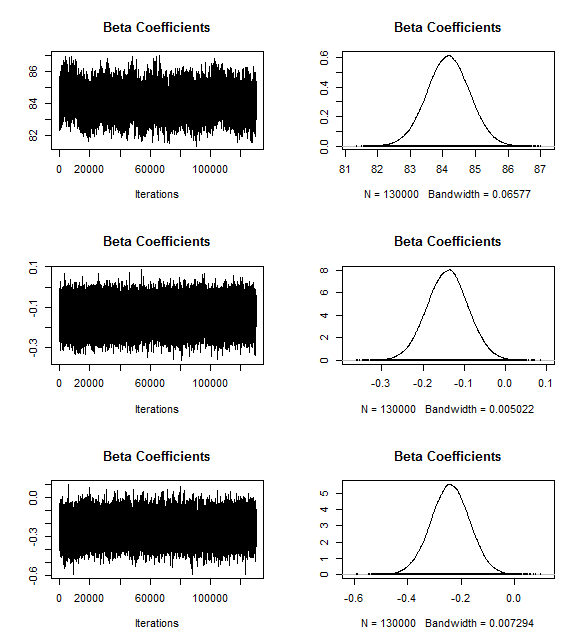
\includegraphics[scale=.9]{trace_plots.png}
\label{lab:trace_plots}
\end{figure}

Figures of the posterior median and standard deviation of the spatial random effects can be found in Figure \ref{lab:med_sd}. From these figures we see that the highest posterior medians are found at the top of Michigan and the least of which are clustered together near the north-west, where our preliminary graduation plot exhibited lower graduation rates. We also see that the greatest standard deviations are at the northern part of Michigan and the smallest are located near the center of Michigan. However, when we construct our 95\% credible intervals for each of the 83 counties, we find that all intervals contain 0, indicating that there are no significantly positive or negative spatial random effects in play.

\begin{figure}[h!]
\caption{Median (left) and standard deviations (right) of the spatial random effects using an improper CAR model}
\centering
\begin{minipage}{.5\textwidth}
  \centering
  \scalebox{.81}{
 \trimbox{1cm 2cm 0cm 0cm}{\input{"med_spat_rand.tex"}}
 }
\end{minipage}%
\begin{minipage}{.5\textwidth}
  \centering
  \scalebox{.81}{
 \trimbox{0cm 2cm -1cm 0cm}{\input{"sd_spat_rand.tex"}}
 }
\end{minipage}

\label{lab:med_sd}
\end{figure}


Next, we create a Bayesian spatial proper CAR model which yields the results from Table \ref{tab:proper_car}. The results of this procedure are very similar to those of the improper CAR model. The covariates are all significant, though this model suggests a slightly stronger effect for the percentage of black students and a weaker effect for the percentage of students economically disadvantaged. 

\begin{table}
  \caption{Results of using a proper CAR model on the Michigan county areal data} 
  \label{tab:proper_car}
  \centering 
 \begin{tabular}{||c c c c||} 
 \hline
 Coefficients & Estimate & Standard Error & P-Value\\ [0.5ex] 
 \hline\hline
 Intercept & 84.47 & 0.775 & $<$ 2.2e-16 \\ 
 \hline
 \% Economically Disadvantaged & -0.114 & 0.0526  & 0.0289 \\
 \hline
 \% Black & -0.275 & -0.0717 & 0.0001 \\[0.5ex] 
 \hline
\end{tabular}
\end{table}

Additionally, we fit a SAR model with nearly identical summary results, as seen in Table \ref{tab:sar}.

\begin{table}
  \caption{Results of using a SAR model on the Michigan county areal data} 
  \label{tab:sar}
	\centering
 \begin{tabular}{||c c c c||} 
 \hline
 Coefficients & Estimate & Standard Error & P-Value\\ [0.5ex] 
 \hline\hline
 Intercept & 84.288 & 0.745 & $<$ 2.2e-16 \\ 
 \hline
 \% Economically Disadvantaged & -0.121& 0.05155 & 0.0184 \\
 \hline
 \% Black & -0.275 & -0.0715 & 0.0001 \\[0.5ex] 
 \hline
\end{tabular}
\end{table}

Finally, we fit a spatial model to the number of students graduating, modeled as Poisson data with both spatial and non-spatial random effects. Here, the mean number of students graduating in each county is equal to expected counts multiplied by relative risk. We use a burn in of 30,000 and an overall sample of 170,000 to relate the log mean of the Poisson distribution to the covariates. As a result, we use the log of expected counts as an offset when modeling how the log of relative risk varies with the covariates. The results of the model can be seen in Table \ref{tab:poi}. Since the absolute values of the Geweke diagnostics are less than 2, and the effective sizes are fairly large, it appears that the estimates converged to the desired posterior distributions.

\begin{table}
  \caption{Results of a Poisson, ``disease-mapping" approach to graduation rates} 
  \label{tab:poi}
\centering
 \begin{tabular}{||c c c c c c||} 
 \hline
 Covariate & Median & 2.5 & 97.5 & Effective Size & Geweke Diag.\\ [0.5ex] 
 \hline\hline
 Intercept & -0.1566 & -0.1691 & -0.144 & 2460 & -1.6 \\ 
 \hline
 \% Econ. Disadvantaged & -0.0016 & -0.0033 & 0.0002 & 991 &-0.5 \\
 \hline
 \% Black & -0.0016 & -0.0033 & 0.0002 & 633 & 0.9\\
 \hline
 tau2 & 0.023 & 0.0012 & 0.0049 & 3600 & 1.0\\ 
\hline
 sigma2 & 0.0013 & 0.0008 & 0.0023 & 6595 & 0.5\\ [0.5ex] 
 \hline
\end{tabular}
\end{table}

We visualize the estimated propensity to graduate through another choropleth map in Figure \ref{lab:post_med_poi}. The propensities are largely consistent with our preliminary graduation rates. We find a lower propensity to graduate high school in the north-west region (though not at the very top of the map) of Michigan, and higher propensities in the Northern tip of Michigan. 

\begin{figure}[h!]
\caption{Estimated propensity to graduate Michigan high schools (left), posterior medians of spatial random effects for each county using a disease-mapping approach (right), and those effects that are statistically significant (bottom)}
\centering
\begin{minipage}{.5\textwidth}
  \centering
  \scalebox{.81}{
 \trimbox{1cm 2cm 0cm 0cm}{\input{"propensity.tex"}}
 }
\end{minipage}%
\begin{minipage}{.5\textwidth}
  \centering
  \scalebox{.81}{
 \trimbox{0cm 2cm -1cm 0cm}{\input{"post_med_poi.tex"}}
 }
\end{minipage}

\begin{minipage}{.5\textwidth}
  \centering
  \scalebox{.81}{
 \trimbox{0cm 2cm -1cm 0cm}{\input{"sig_effects.tex"}}
 }
\end{minipage}
\label{lab:post_med_poi}
\end{figure}

In Figure \ref{lab:post_med_poi} (right), we find the plotted posterior medians of spatial random effects. Compared with the previous map in Figure \ref{lab:med_sd}, this is less smooth across large patches of counties. We still observe similar spatial patterns, however: positive effects at the northern tip and negative effects in the north-west and center regions. We note, however, that the medians in this figure exhibit less deviation from 0, indicating weaker spatial random effects. From the bottom of Figure \ref{lab:post_med_poi}, we notice two counties with statistically significant spatial random effects, both of which were negative. These counties, Manistee and St. Clair, exhibit lower graduation rates than we would expect given the percent of their students who are African-American and economically disadvantaged.

\section{Conclusions}
In conclusion, we notice a large-scale association between Michigan county-level graduation rates and the percentage of students who are African-American or considered economically disadvantaged. On average, those counties that exhibit higher-than-average proportions of black students, or higher-than-average proportions of economically disadvantaged students tend to have lower high school graduation rates. A county that has 10\% more economically disadvantaged students than average tends to have a graduation rate 1.1\% less than the state average. A county with 10\% more African-American students actually has about a 2.8\% negative disparity in graduation rate from the state average.

Michigan high school graduation rates do tend to exhibit spatial correlation across counties based on the results of our models. With the exception of the very northern tip of Michigan, which exhibits very high graduation rates, the north-west areas of Michigan tend to have lower rates of graduation. Alternatively, the south-east regions of Michigan exhibit higher rates of graduation.

In two instances, specifically Manistee county and St. Clair county, the graduation rates are even lower than we would expect based on their proportions of African-American and economically disadvantaged students.


\section{References}

\indent [1] Bureau of Labor Statistics  (2015). Employment Situation Summary. Retrieved from [http://www.bls.gov/emp/ep\_chart\_001.htm].

[2] Bureau of Labor Statistics  (2015). Earnings and unemployment rates by educational attainment. Retrieved from [http://www.bls.gov/emp/ep\_chart\_001.htm].

[3] U.S. Department of Education, EDFacts/Consolidated State Performance Reports (2015)

\end{document}







